\documentclass[aspectratio=169,12pt,spanish]{beamer}
\usepackage[T1]{fontenc}
\usepackage[spanish]{babel}
%\usepackage{natbib}

\usepackage{wrapfig}

%\usepackage{multicol}
%\usepackage{mathtools}

\usepackage[normalem]{ulem}

\usepackage{pgf,tikz}
\usetikzlibrary{matrix}
\usetikzlibrary{arrows}

%\usepackage{wrapfig}
\mode<presentation>
\usefonttheme{professionalfonts}
\usetheme{Darmstadt}
\usecolortheme{orchid}
\useoutertheme{default}
\setbeamertemplate{headline}{}

\renewcommand{\baselinestretch}{1.1}

%gets rid of bottom navigation bars
\setbeamertemplate{footline}[page number]

%gets rid of navigation symbols
\setbeamertemplate{navigation symbols}{}

%\frameframe{none} % No default frame

%\setlength{\framewidth}{8.7in} \setlength{\frameheight}{7.2in}

\parindent 0pt
\setlength{\parskip} {1ex plus 0.5ex minus 0.2ex}


\usepackage[bbgreekl]{mathbbol}
\usepackage{amssymb, amsthm, amsmath}
\usepackage{bm}

\newtheorem{ejercicio}{Ejercicio}

\DeclareSymbolFontAlphabet{\mathbb}{AMSb}
\DeclareSymbolFontAlphabet{\mathbbl}{bbold}

\usepackage{multicol}
\usepackage{colortbl}
\usepackage{lmodern}
\usepackage{tabularx}
\usepackage{multirow}
\usepackage{stmaryrd}
\usepackage{color}
\usepackage{graphicx}
\usepackage{hyperref}

\graphicspath{ {../../images} }
\usepackage{listings}
\lstset{
  basicstyle=\ttfamily,
  columns=fullflexible,
}

\usepackage{url}
\usepackage{multicol}
\usepackage{dsfont}

% Bold symbols for vectors and matrices
\newcommand{\xstar}{\bm{x}^{\star}}
\newcommand{\alphab}{\bm{\alpha}}
\newcommand{\ab}{\bm{a}}
\newcommand{\bb}{\bm{b}}
\newcommand{\cb}{\bm{c}}
\newcommand{\db}{\bm{d}}
\newcommand{\eb}{\bm{e}}
\newcommand{\gb}{\bm{g}}
\newcommand{\mb}{\bm{m}}
\newcommand{\pb}{\bm{p}}
\newcommand{\qb}{\bm{q}}
\newcommand{\rb}{\bm{r}}
\newcommand{\ssb}{\bm{s}}
\newcommand{\ub}{\bm{u}}
\newcommand{\vb}{\bm{v}}
\newcommand{\wb}{\bm{w}}
\newcommand{\xb}{\bm{x}}
\newcommand{\yb}{\bm{y}}
\newcommand{\zb}{\bm{z}}

\newcommand{\Ab}{\bm{A}}
\newcommand{\Bb}{\bm{B}}
\newcommand{\Cb}{\bm{C}}
\newcommand{\Db}{\bm{D}}
\newcommand{\Eb}{\bm{E}}
\newcommand{\Fb}{\bm{F}}
\newcommand{\Gb}{\bm{G}}
\newcommand{\Hb}{\bm{H}}
\newcommand{\Ib}{\bm{I}}
\newcommand{\Id}{\bm{I}}
\newcommand{\Kb}{\bm{K}}
\newcommand{\Lb}{\bm{L}}
\newcommand{\Mb}{\bm{M}}
\newcommand{\Pb}{\bm{P}}
\newcommand{\Qb}{\bm{Q}}
\newcommand{\Rb}{\bm{R}}
\newcommand{\Sb}{\bm{S}}
\newcommand{\Tb}{\bm{T}}
\newcommand{\Ub}{\bm{U}}
\newcommand{\Vb}{\bm{V}}
\newcommand{\Wb}{\bm{W}}
\newcommand{\Xb}{\bm{X}}
\newcommand{\Yb}{\bm{Y}}
\newcommand{\Zb}{\bm{Z}}
\newcommand{\Lambdab}{\bm{\Lambda}}
\newcommand{\cero}{\bm{0}}

% Rings and fields
\newcommand{\A}{\mathbb{A}}
\newcommand{\Z}{\mathbb{Z}}
\newcommand{\Q}{\mathbb{Q}}
\newcommand{\C}{\mathbb{C}}
\newcommand{\R}{\mathbb{R}}
\newcommand{\K}{\mathbb{K}}
\newcommand{\N}{\mathbb{N}}

\newcommand{\borel}{{\mathcal B}}
\newcommand{\pmom}{{\rho_{\text{mom}}}}
\newcommand{\MX}{{\mathcal{M}(X)}}


% Inner product
\newcommand{\innerl}[2]{\langle #1, #2 \rangle}
\newcommand{\inner}[2]{#1 \boldsymbol{\cdot} #2}
\newcommand{\innerTrace}[2]{#1 \bullet #2}

% Symmetric and positive definite matrices
\newcommand{\Splusplusn}{{\mathcal S_{++}^n}}
\newcommand{\Splusn}{{\mathcal S_+^n}}
\newcommand{\Splus}{{\mathcal S_+}}
\newcommand{\Sym}{{\mathcal S}}
\newcommand{\Symn}{{\mathcal S^n}}

% Cones
\newcommand\CC{\mathcal{C}}
\DeclareMathOperator{\cone}{cono}
\DeclareMathOperator{\conv}{conv}
\DeclareMathOperator{\supp}{supp}


% Spectrahedron
\newcommand{\eLL}{{\mathcal L}}

% Matrices and vectors over R or C
\newcommand{\Rnn}{\R^{n\times n}}
\newcommand{\Cnn}{\C^{n\times n}}
\newcommand{\Rn}{\R^{n}}
\newcommand{\Rm}{\R^{m}}


% Math operators
\DeclareMathOperator{\Tr}{Tr}
\DeclareMathOperator{\tr}{Tr}
\DeclareMathOperator{\interior}{int}
\DeclareMathOperator{\rank}{rank}
\DeclareMathOperator{\diag}{diag}

\newcommand\one{\mathds{1}} 

\pagestyle{empty}

\begin{document}

%------------------------------------------------------------------

\begin{frame}

 \begin{center}

\Large\textbf{Optimización Semidefinida} \\
\large\textbf{Clase 02 - Soluciones básicas en programación lineal}
%\vspace{0.5cm}

% \textit{Santiago Laplagne} \\
%slaplagn@dm.uba.ar \\


%\vspace{0.5cm}
%{\small Trabajo en progreso en conjunto con \emph{Jose Capco} (Universit\"at Innsbruck) y \emph{Claus Scheiderer} %(Universit\"at Konstanz).} \\

\vspace{1cm}
 Segundo Cuatrimestre 2021
 \\
 {\small Facultad de Ciencias Exactas y Naturales, UBA}
 \end{center}

\end{frame}

%------------------------------------------------------------------

\begin{frame}
\frametitle{Puntos extremales}

Ya vimos geométricamente que la solución óptima de un problema de programación lineal se encuentra en una esquina de la región factible. Veamos ahora diferentes formas de formalizar la idea de esquina.

\begin{definition}
  Dado un poliedro $P$, un vector $\xb \in P$ es un \emph{punto extremal} de $P$ si no puede escribirse como combinación convexa de dos puntos de $P$ distintos de $\xb$. Es decir, si no existen dos vectores $\yb, \zb \in P$, ambos diferentes de $\xb$, y un escalar $\lambda \in [0, 1]$ tales que
  $$\xb = \lambda \yb + (1-\lambda) \zb.$$
\end{definition}


\end{frame}

%------------------------------------------------------------------

\begin{frame}
\frametitle{Puntos extremales}

\begin{center}
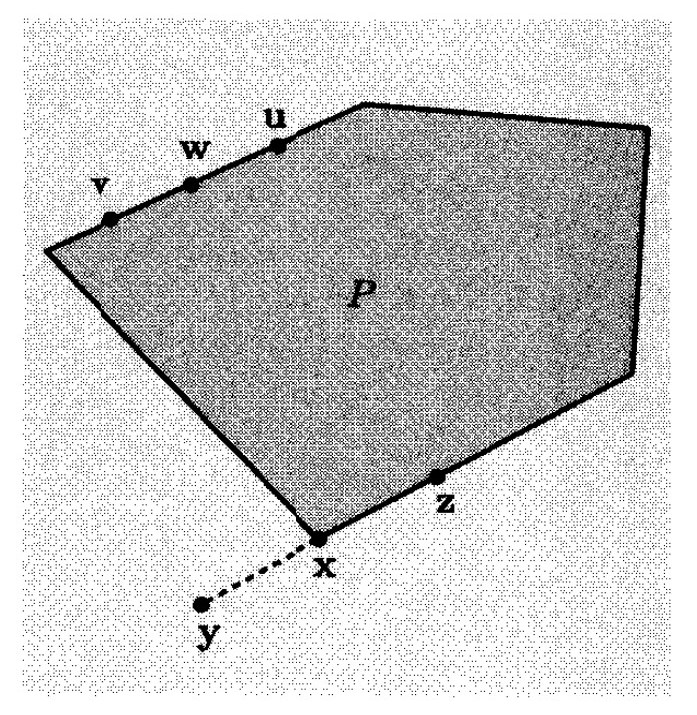
\includegraphics[scale=.2]{extremePoint.jpg}
\end{center}

El punto $\wb$ no es un punto extremal porque es una combinación convexa de $\ub$ y $\vb$. Por el contrario $\xb$ es un punto extremal. Si $\xb = \lambda \yb + (1-\lambda) \zb$ y $\lambda \in [0,1]$ entonces $\yb \not\in P$ o $\zb \not\in P$ o $\xb = \yb$ o $\xb = \zb$.

Pregunta: ¿cuáles son los puntos extremales de un conjunto no convexo?
\end{frame}

%------------------------------------------------------------------

\begin{frame}
\frametitle{Vértices}

Otra posibilidad es considerar a los puntos que son solución óptima única de un problema de programación lineal.

\begin{definition}
Dado un poliedro $P \subset \R^n$, un vector $\xb \in P$ es un \emph{vértice} de $P$ si
existe $\cb \in \R^n$ tal que
$$\inner{\cb}{\xb} < \inner{\cb}{\yb}$$
para todo $\yb \in P$, $\yb \neq \xb$.
\end{definition}

Es decir, $\xb$ es un vértice de $P$ si $P$ está de un lado de un hiperplano (el hiperplano $\{\yb \in \R^n \mid \inner{\cb}{\yb} = \inner{\cb}{\xb}\}$) que toca a $P$ solo en $\xb$.


\end{frame}

%------------------------------------------------------------------

\begin{frame}
\frametitle{Vértices}

\begin{center}
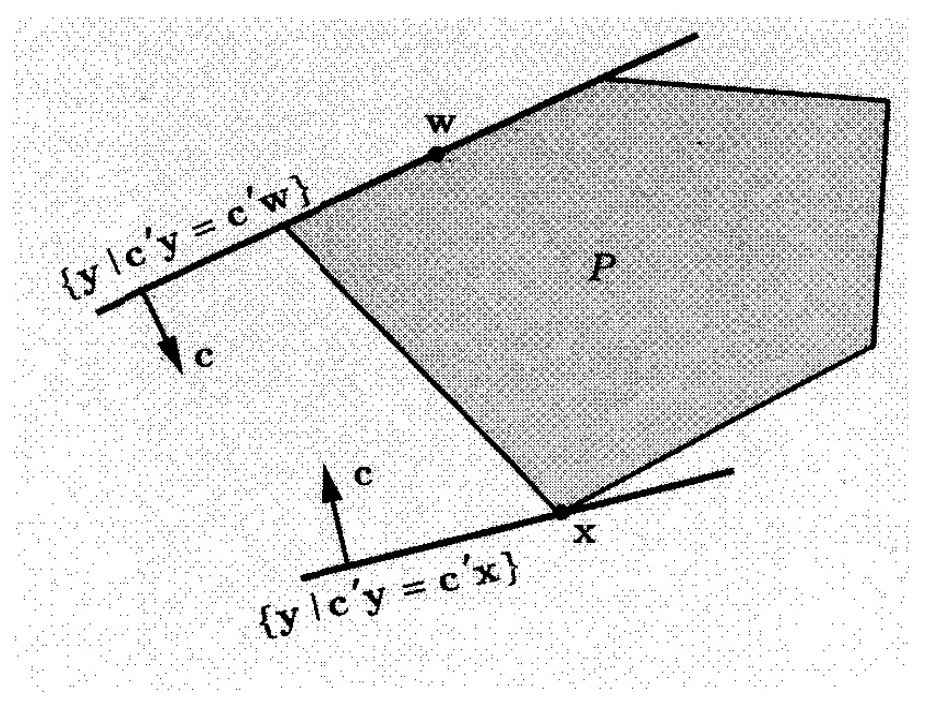
\includegraphics[scale=.2]{vertex.jpg}
\end{center}

El punto $\xb$ es un vértice porque hay un hiperplano (una línea recta) que toca a $P$ solo en $\xb$.

Por el contrario $\wb$ no es un vértice porque no hay ningún hiperplano que toque a $P$ solo en $\wb$.

\end{frame}

%------------------------------------------------------------------

\begin{frame}
\frametitle{Verificación algorítmica}

Una desventaja de estas definiciones geométricas es que dado un poliedro $P$ definido como intersección de hiperplanos y semiespacios, y un punto $\xb$, no es fácil verificar si se cumplen las definiciones. Veremos a continuación una definición alternativa que podemos verificar fácilmente.

\end{frame}

%------------------------------------------------------------------

\begin{frame}
\frametitle{Restricciones activas}

Consideramos un poliedro $P$ definido por igualdades y desigualdades lineales,
$$
\begin{cases}
\inner{\ab_i}{\xb} \ge b_i, & i \in M_1 \\
\inner{\ab_i}{\xb} \le b_i, & i \in M_2 \\
\inner{\ab_i}{\xb} = b_i, & i \in M_3,
\end{cases}
$$
donde $M_1, M_2, M_3$ son conjuntos finitos de índices, $\ab_i$ son vectores en $\R^n$ y $b_i$ son escalares.

\begin{definition}
Si un vector $\xb^\star$ satisface una igualdad $\inner{\ab_i}{\xb^\star} = b_i$ para alg\'un $i \in M_1$, $M_2$ o $M_3$, decimos que la restricción correspondiente está \emph{activa} en $\xb^\star$.
\end{definition}


\end{frame}

%------------------------------------------------------------------

\begin{frame}
\frametitle{Restricciones activas}

\begin{center}
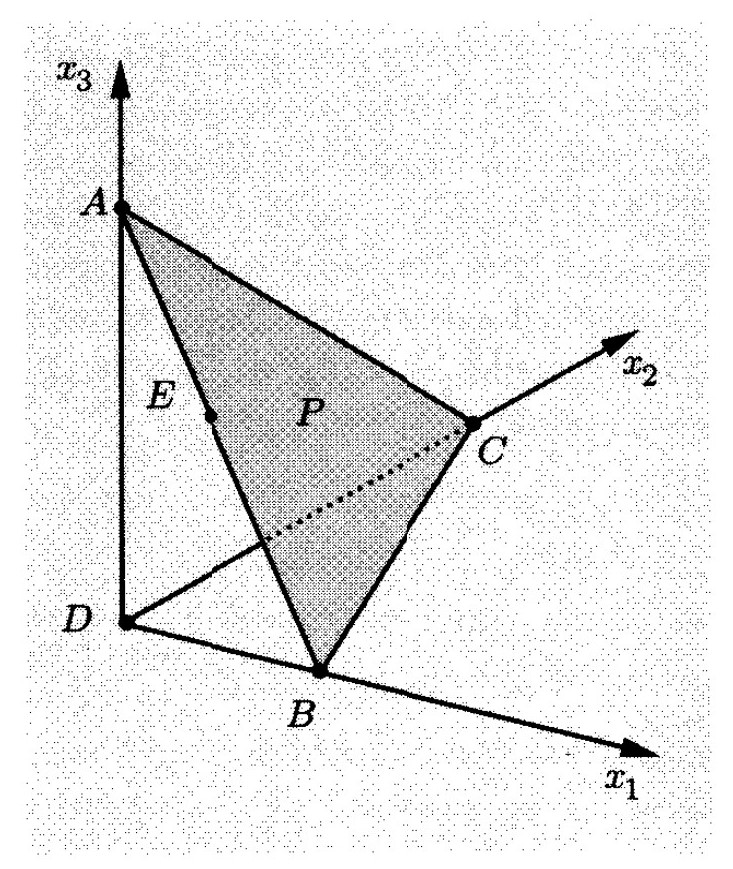
\includegraphics[scale=.2]{activeConstraints.jpg}
\end{center}

Para el poliedro $P = \{(x_1, x_2, x_3) \in \R^3 \mid x_1 + x_2 + x_3 = 1, \xb \ge 0\},$
\begin{itemize}
\item hay tres restricciones activas en los puntos $A$, $B$, $C$ y $D$.
\item hay solo dos restricciones activas en $E$: $x_1 + x_2 + x_3 = 1$ y $x_2 = 0$.
\end{itemize}

\end{frame}

%------------------------------------------------------------------

\begin{frame}
\frametitle{Soluciones básicas y soluciones básicas factibles}

En $\R^n$, si hay $n$ condiciones activas, $\xb^\star$ es solución de un sistema de $n$ ecuaciones con $n$ incógnitas. Si las $n$ ecuaciones son linealmente independientes, el sistema tiene solución única. Teniendo esto en cuenta, hacemos la siguiente definición.

\begin{definition}
Sea un poliedro $P$ definido por igualdades y desigualdades lineales y $\xb^\star \in \R^n$.
\begin{enumerate}
\item El vector $\xb^\star$ es una \emph{solución básica} si
\begin{enumerate}
\item todas las igualdades están activas,
\item de todas las restricciones activas, hay $n$ de ellas que son linealmente independientes
\end{enumerate}
\item Si $\xb^\star$ es una solución básica que satisface todas las restricciones, decimos que $\xb^\star$ es una \emph{solución básica factible}.
\end{enumerate}
\end{definition}

\end{frame}

%------------------------------------------------------------------

\begin{frame}
\frametitle{Soluciones básicas y soluciones básicas factibles}

Observamos que en el conjunto de restricciones podemos reemplazar una igualdad $\inner{\ab}{\xb} = b$ por dos desigualdades $\inner{\ab}{\xb} \le b$ y $\inner{\ab}{\xb} \ge b$, obteniendo un problema equivalente. Por lo tanto, la condición de ser solución básica depende de cómo está formulado el problema.

\end{frame}

%------------------------------------------------------------------

\begin{frame}
\frametitle{Punto extremo $\iff$ Vértice $\iff$ Solución básica factible}

\begin{theorem}
Dado un poliedro $P$ no vacío y un vector $\xb^\star \in P$, las siguientes propiedades son equivalentes:
\begin{enumerate}
\item $\xb^\star$ es un punto extremo de $P$,
\item $\xb^\star$ es un vértice de $P$,
\item $\xb^\star$ es una solución básica factible de $P$.
\end{enumerate}
\end{theorem}

\textbf{Demostración.} Ver apunte o \cite[Teorema 2.3]{Bertsimas1997}.
\end{frame}

%------------------------------------------------------------------

\begin{frame}
\frametitle{Independencia de las ecuaciones}

Las dos primeras definiciones son definiciones geométricas y solo dependen del conjunto $P$ y no de las ecuaciones que lo definen. Por la equivalencia, obtenemos que la condición de solución básica factible tampoco depende de las ecuaciones que definen $P$, a diferencia de las soluciones básicas que sí pueden depender.

\end{frame}

%------------------------------------------------------------------

\begin{frame}
\frametitle{Cantidad finita de soluciones}

Obtenemos el siguiente corolario simple pero muy importante.

\begin{corollary}
Dado un conjunto finito de restricciones lineales (igualdades o desigualdades), la cantidad de soluciones básicas y soluciones básicas factibles es siempre finita.
\end{corollary}

\textbf{Observación}
Si bien la cantidad de soluciones básicas es siempre finita, puede ser una cantidad muy grande. Por ejemplo, el cubo
$$
\{\xb \in \R^n \mid 0 \le x_i \le 1, 1 \le i \le n\}
$$
está definido por $2n$ ecuaciones y tiene $2^n$ soluciones básicas factibles.
Esto hace que en la práctica, si bien podemos evaluar la función a optimizar en todas las soluciones básicas factibles para encontrar el óptimo, puede ser un método muy ineficiente.


\end{frame}

%------------------------------------------------------------------

\begin{frame}
\frametitle{Poliedros en forma estándar}

Un poliedro en forma estándar está definido por las siguientes ecuaciones:
$$
P = \{\xb \in \R^n : \Ab\xb = \bb, \xb \ge 0\},
$$
donde $\Ab \in \R^{m \times n}$, es decir el poliedro está definido por $m$ igualdades y $n$ desigualdades $x_i \ge 0$.
Eliminando filas redundantes de $\Ab$, podemos suponer que las $m$ filas de $\Ab$ son linealmente independientes, y por lo tanto debe ser $m \le n$.

\end{frame}


%------------------------------------------------------------------

\begin{frame}
\frametitle{Construcción de soluciones básicas}


Recordemos que en una solución básica debe haber $n$ restricciones linealmente independientes activas, y más aún, todas las restricciones de igualdad se deben cumplir, lo que nos da $m$ restricciones.

Como $m \le n$, para obtener $n$ restricciones activas, debemos elegir $n - m$ variables $x_i$ y darles valor $0$, para activar las correspondientes $n-m$ desigualdades $x_i \ge 0$. Es decir, para construir soluciones básicas:
\begin{itemize}
\item Tenemos $m$ restricciones de igualdad activas.
\item Tomamos $n - m$ restricciones $x_i = 0$ para completar $n$ restricciones activas.
\end{itemize}

Debemos tener cuidado que no cualquier elección de las $n-m$ variables $x_i$ nos va a dar un conjunto de $n$ restricciones linealmente independientes. En el siguiente teorema vemos las condiciones que tenemos que cumplir.


\end{frame}

%------------------------------------------------------------------

\begin{frame}
\frametitle{Construcción de soluciones básicas}

\begin{theorem}
Consideremos las restricciones $\Ab\xb = \bb$ y $\xb \ge 0$, donde suponemos que las $m$ filas de $\Ab \in \R^{m \times n}$ son linealmente independientes.
Un vector $\xb^\star \in \R^n$ es una solución básica si y solo si $\Ab\xb^\star = \bb$ y existen índices $B(1), \dots, B(m)$ tales que
\begin{enumerate}
\item las columnas $\Ab_{B(1)}, \dots, \Ab_{B(m)}$ son linealmente independientes,
\item si $i \neq B(1), \dots, B(m)$, entonces $x_i = 0$.
\end{enumerate}
\end{theorem}

\textbf{Demostración.} Ver \cite[Teorema 2.4]{Bertsimas1997}.

\end{frame}

%------------------------------------------------------------------

\begin{frame}
\frametitle{Construcción de soluciones básicas}

Este teorema nos da un procedimiento para construir soluciones básicas de un poliedro en forma estándar.

\begin{enumerate}
\item Elegir $m$ columnas linealmente independientes $\Ab_{B(1)}, \dots, \Ab_{B(m)}$.
\item Fijar $x_i = 0$ para todo $i \neq B(1), \dots, B(m)$.
\item Resolver el sistema de $m$ ecuaciones $\Ab\xb = \bb$ para las variables $x_{B(1)}, \dots, x_{B(m)}$.
\end{enumerate}

Recordemos que en una matriz el rango fila y el rango columna coinciden, por lo tanto siempre podemos encontrar $m$ columnas independientes en $\Ab$.

Si una solución básica construida siguiendo el procedimiento cumple que todas sus coordenadas son no-negativas, entonces es una solución básica factible. Recíprocamente, podemos encontrar todas las soluciones básicas factibles de esta forma.


\end{frame}

%------------------------------------------------------------------

\begin{frame}
\frametitle{Variables básicas y columnas básicas}

\begin{block}{Variables básicas}
Si $\xb$ es una solución básica, llamamos \emph{variables básicas} a las variables $x_{B(1)}, \dots, x_{B(m)}$ y \emph{no-básicas} a las demás variables.
\end{block}

\begin{block}{Columnas básicas}
Llamamos \emph{columnas básicas} a las columnas $\Ab_{B(1)}, \dots, \Ab_{B(m)}$. Como son linealmente independientes, forman una base de $\R^m$. \end{block}

Llamamos \emph{matriz base asociada} a la matriz formada por estas columnas:
$$
\Bb = \begin{pmatrix} \vert & & \vert \\ \Ab_{B(1)} & \dots & \Ab_{B(m)} \\ \vert & & \vert \end{pmatrix}.
$$

\end{frame}

%------------------------------------------------------------------

\begin{frame}
\frametitle{Soluciones degeneradas}

Observamos que dos conjuntos distintos de variables básicas pueden dar la misma solución básica, si algunas de las variables básicas valen también $0$. En este caso, decimos que la solución es \emph{degenerada}.

Para simplificar el desarrollo de este tema, supondremos siempre que todas las soluciones básicas del problema son no-degeneradas.


\end{frame}

%------------------------------------------------------------------

\begin{frame}
\frametitle{Referencias}

\bibliographystyle{apalike}
\bibliography{../../latex/optimizacion}

\end{frame}

\end{document}
